
\subsection{Data Management}
\label{sec:datamanager}

% Most of the following are taken from Yu Ma's dissertation
Data management needs for \ac{swim} are complex due to the nature of
computation codes involved. Many codes have established some basic 
data staging pipelines and set up preferred I/O formats
to use data management tools like MDSplus \cite{mdsplus}. 
% need to find reference for mdsplus

% IPS doc stuff
Predefined directory structures for running simulations can be used
to keep track of data files directly. The Integrated Plasma Simulator (IPS)
Design Description document proposes the following directory layout of control 
and input files in user space. 
How to set up and populate such a simulation directory is yet to be 
discussed. 
% Include the Proposed Simulation File Tree here.
\newpage
\begin{verbatim}
IPS_run_XYZ
  |-- simulation_setup
    |-- system_config
    |-- simulation_wide_data
      |-- simulation_control_file (this is a file not a directory)
      |-- initial_plasma_state (t0) (this is a file not a directory)
      |-- machine_definition (may be empty for now)
      |-- simulation_events_waveforms 
      (scheduled events, source and control waveforms)
    |-- component_inputs
      |-- RF
        |-- RF_component (the component may need generic files)
          |-- RF_config
          |-- RF_required_list
          |-- RF_outfile_list
        |-- code_inputs (code specific files e.g. AORSA)
          |-- AORSA_required_list
          |-- AORSA_outfile_list
          |-- Standard AORSA input files  ...
      |-- FokkerPlanck
        |-- FP_component
          |-- FP_config
          |-- FP_required_list
          |-- FP_outfile_list
        |-- code_inputs (code specific input files e.g. CQL3D)
          |-- CQL3D_required_list
          |-- CQL3D_outfile_list
          |-- Standard CQL3D input files  ...
      ...		    
      |-- <other components> ...

  |-- simulation_results
    |-- history
      |-- t0 (identifier in milliseconds)
        |-- plasma_state
        |-- components
          |-- RF
          |-- Fokker Planck
          ...
          |-- <other components>
      |-- t1 (identifier in milliseconds)
        |-- plasma_state
        |-- components
          |-- RF
          |-- FokkerPlanck
          ...
          |-- <other components>
      ...		
      |-- tN ...<other time steps>
    |-- restart
      |-- t0 (identifier in milliseconds)
        |-- RF
          |-- input_files
          |-- internal_state
        |-- Fokker Planck
          |-- input_files
          |-- internal_state
        ...		    
        |-- <other components>
      |-- t1 (identifier in milliseconds)
        |-- RF
        |-- Fokker Planck
        ...
        |-- <other components> ...
      ...	
      |-- tN ...<other time steps> 
      
  |-- work
    |-- plasma_state (current plasma state tn)
    |-- RF
      |-- RF_component (the component may need generic files)
        |-- RF_config
        |-- RF_required_list
        |-- RF_outfile_list
        |-- RF_log
      |-- code_inputs (code specific input files e.g. AORSA)
        |-- AORSA_required
        |-- AORSA_outfile_list
        |-- AORSA standard input files ...
      |-- RF_component_script (?)
      |-- executable (?)
      |-- code_outputs
        |-- AORSA standard input files ...
        |-- AORSA_log
      |-- scratch
    ...	    
    |-- <other components> ...
\end{verbatim}
%
\newpage

A comprehensive predefined directory structure can be  
straightforward for locating data files of a particular simulation run, 
but could become cumbersome as the data volume grows. Supplementary
metadata management based on \ac{rdbms} techniques is beneficial in this 
case, where more sophisticated search queries and more flexible 
data storage schemas are supported. 
Additionally, new data sharing and manipulation requirements continue to 
emerge as the community framework evolves. 
For example, when different computational
components are combined to work together and interact with each other under a
distributed environment, input and output files are often shared and
duplicated among them, and likely in groups. The ability to define
an aggregate of files, and subsequently archive, locate, and retrieve them
individually or as a bundle, is beyond the scope of data management tools
already in use. Moreover, external notification mechanisms like event systems
will be deployed in the framework for different components to communicate with
each other on information like computation status and file operations,
a desired data management system should in turn interact with such an
external system for not only information exchange but also logging purpose.

For the system flexibility and extensibility, a customized data management
solution for \ac{swim} is developed under Obsidian \cite{obsidian} composable
architecture. This data manager mainly subscribes to the event channel and
responds accordingly to various data management requests described in event
messages. In addition, all related event messages are archived in
the back-end MySQL RDBMS for logging purpose, together with
Event specific metadata as defined in Table \ref{eventmd}, which are
available as query conditions for looking up particular events.
\begin{table}
\begin{center}
\begin{tabular}{|c|c|} \hline
\multicolumn{2}{|c|}{EventMD} \\ \hline \hline
EventID     &   Unique event ID \\ \hline
topic       &   Event topic as required by the event channel \\ \hline
ts          &   Timestamp of when the event is published    \\ \hline
publisher   &   User ID of who published the event      \\ \hline
component   &   Computation component ID which published the event \\ \hline
host        &   Machine host name from where the event is published \\ \hline
action      &   Progress notification or computational request  \\ \hline
message     &   Additional arbitrary user messages  \\ \hline
\end{tabular}
\caption{\label{eventmd} FSP Event Metadata}
\end{center}
\end{table}

Two initial types of data management requests have been identified as requiring
further actions from the data manager: one for archiving physical metadata of
computation component I/O files, the other for aggregating files in collections
as specified by users. Once every file of computational significance has been
recorded in the metadata database through Obsidian 
{\it Physical Location Tracker}, 
arbitrary aggregates of these files can be defined through
{\it Logical Collection Manager}, though most commonly according to job
executions of computation components.
As an example depicted in Figure \ref{fspcol}, several input and output files
are involved in two runs of the same computation. Two file collections
can then be respectively defined for those from each run,
enabling later queries to find basic metadata about all files in the same run
as a given file.
\begin{figure}
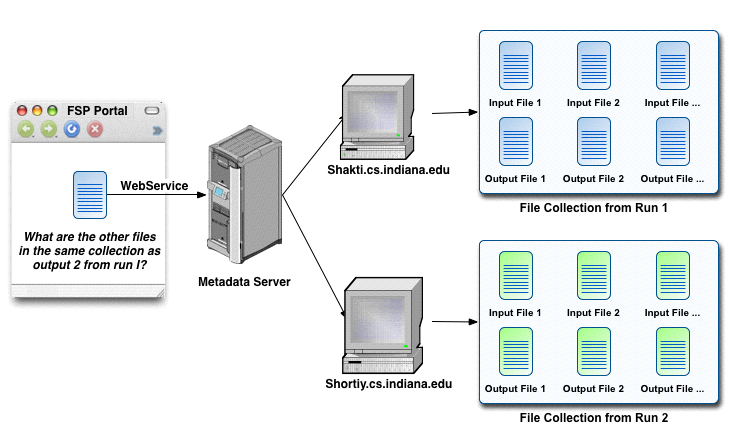
\includegraphics[scale=0.55]{file_collection.jpg}
\caption{FSP Example of Defining I/O File Aggregations}
\label{fspcol}
\end{figure}
A web service interface has been provided by the \ac{swim} data manager in
WSDL descriptions to enable interactions between the Portal and the back-end
metadata database. 
%
%\ac{swim} (like most modern scientific simulation projects) needs the ability to
%store, track, and query results. The \ac{swim} framework provides a data manager
%called Obsidian as a portlet or a standalone web service. 
However, A \ac{swim} user does not {\em have} to use the data manager and can
use another data management method like directory/file naming conventions
in place or along with it.

The data manager is used for internal information management in the portal
but end users need not deal with that.  In general three types of metadata
are defined:
        \begin{enumerator}
        \item Notifications and events published by any component or portal utility
        \item File announcements and creation. Metadata includes name, location,
              user ID of the file owner, which component created it, timestamp,
              purpose of the file, and a \ac{swim} job ID.
        \item Aggregates of files. It is convenient at times to deal with a
              collection of files such as ``all output files from a given \ac{swim}
              run'', instead of each file individually. Aggregates can be
              overlapping with a single file belonging to several at the same
              time. So ``aggregate'' does not imply the collection is a
              directory or even on the same machine.
        \end{enumerator}
        
Portal pages have been written that use the event data management to
display published events of types notification, data, and job management
dynamically. Additionally there is a portal page with a simple \ac{gui} that allows
users to enter complex queries, such as a request to view all files
belonging to user bramley created over the past week, which were used as
inputs to an RF component. If a type of query seems likely to be common
it can be added it as a predefined one, available to single users or the
whole project (via the customization capability of portals).
    
Although object storage is a more modern and flexible concept, currently
all the codes and components targeted by \ac{swim} are file-based: consuming
input and name-list files, producing output files. Files are a familiar
concept to most users. \ac{swim} provides some utilities to help coordinate,
track, and locate files.  Even without distributed computing, running
multiple codes as part of an integrated simulation requires file management
beyond what is currently done by the individual codes. The file
specification lists in {\bf SWIM\_ component\_required} and
{\bf SWIM\_component\_results}
consist of one file per line (which can be extended to allow wildcarding
later). With each file listed is an action to take: notify, save, or none.
As the names suggest, the corresponding actions are
\begin{itemize}
    \item {\em notify}: the framework will publish an event that the portal and other
          subscribers can use and act upon it - e.g., start a component that
          requires the file to exist as a prerequisite. 
    \item {\em save}: performs a notify action, and additionally signals the data
          manager to archive the file.
    \item {\em none}: no notification or action is required. The file may be listed
          because it is needed before a component can run.
\end{itemize}
